\subsection{\emph{Gator Tech}}

O projeto \emph{Gator Tech Smart House} é o resultado de mais de cinco anos de pesquisa na área de computação pervasiva e móvel. O objetivo do projeto é criar ambientes assistivos como casas que terão conhecimentos sobre si e sobre seus residentes criando um mapeamento entre o mundo físico, monitoramento remoto e serviços de intervenção~\cite{gatorTech}.

Neste projeto foi desenvolvida uma arquitetura para plataforma de sensores orientada à serviços, o Atlas. A plataforma Atlas é uma combinação de nós de \emph{hardware} e \emph{firmware} executado em um \emph{hardware} e um \emph{middleware} executando na rede, que provê serviços em um ambiente. Juntos, esses componentes permitem que qualquer sensor, atuador ou qualquer outro dispositivo sejam integrados e controlados por meio da interface de um determinado dispositivo. Essa abordagem facilita o desenvolvimento de aplicações que utilizam esses dispositivos~\cite{gatorTechLessons}. 

O Atlas é responsável por obter a representação de serviços dos dispositivos conectados e gerenciar os serviços de modo que as aplicações possam obter e utilizar os serviços facilmente. Na implementação do \emph{Gator Tech}, a camada de serviços foi construída sobre o \emph{framework} OSGi que matém o registro dos serviços de todos os nós conectados. Cada sensor ou atuador é representado no \emph{middleware} Atlas como um pacote de serviços OSGi. Inicialmente esses serviços eram representados em classes Java. Entretanto, a criação desses pacotes não acontecia de forma automática. 

\begin{figure}[ht]
\center
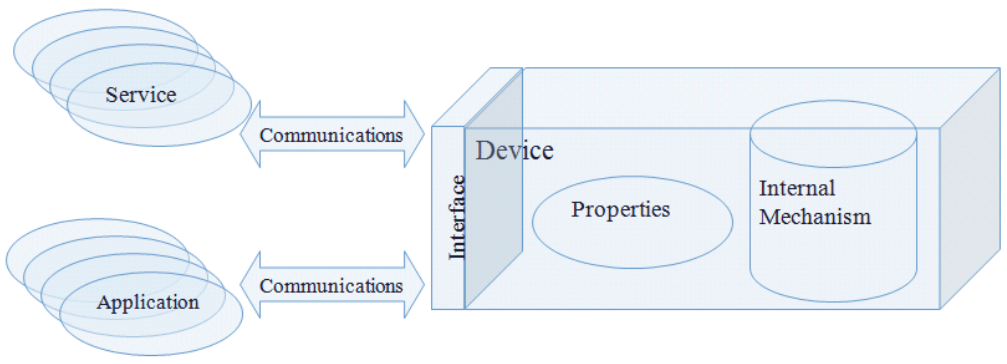
\includegraphics[scale=0.4]{imagens/gatorDDL}
\caption{Caracterização de um Dispositivo~\cite{ddlSpec}}
\label{fig:ddlspec}
\end{figure}

Para cada modelo de sensores e atuadores, era necessário ler a especificação do fabricante, examinar a interface e estudar os protoclos de comunicação. Era necessário ainda, que quem escrevesse o pacote fosse especialista na programação Java e no \emph{framework} OSGi. Com o objetivo de resolver essa complexidade o grupo de pesquisa do Atlas desenvolveu a \emph{Device Description Language}(DDL). Essa linguaguem provê um esquema capaz de descrever a interface dos dispositivos e um processador da linguagem para converter DDL para pacote de serviços OSGi que separa as responsabilidades entre fabricantes de dispositivos, integradores de sistemas e programadores de aplicativos~\cite{gatorTechDDL}.

Na DLL, um dispositivo é caracterizado como uma entidade com propriedades, mecanismo interno e uma interface. Como mostra a figura~\ref{fig:ddlspec}. As propriedades provêem informações a respeito do dispositivo com seu propósito, suas capacidades, fabricante e requisitos operacionais. Essas informações são críticas para a integração do sistema e para programadores de serviços. O mecanismo interno é responsável pela operação do dispositivo e é desconhecido do mundo externo. A interface do dispositivo é a ponte entre o hiato entre o mecanismo interno e o mundo externo. Ela especifica a entrada e saída do dispositivo e provê um guia para aplicações e outros serviços interagirem com o dispositivo.

Os dispositivos foram classificados em três categorias:
\begin{itemize}
	\item Sensor: apenas provê dados de entrada para o usuário externo.
	\item Atuador: apenas aceita dados de saída do usuário externo.
	\item Dispositivo Complexo: provê dados de entrada e aceita dados de saída do usuário externo.
\end{itemize}

Essa classificação genérica tem a disvantagem de ser difícil de ser reutilizada e especializada por diferentes dispositivos, sendo que seus recursos são expostos na forma de serviços por meio da especificação de operações~\cite{ddlSpec}.
